\begin{frame}
	\frametitle{I Terremoti}
	\begin{itemize}
	\item \textbf{Perché avvengono?}
		\begin{itemize}
			\item \pause Movimenti delle placche continentali
		\end{itemize}
	\item \textbf{Come avvengono?}
		\begin{itemize}
			\item \pause Le placche si muovono
			\item \pause L'attrito tra le placche non le fa muovere, ma genera tensione
			\item \pause Quando la tensione supera la resistenza: \textbf{terremoto!}
		\end{itemize}
	\end{itemize}
\end{frame}
\begin{frame}
	\frametitle{Placche planetarie}
	\hspace{1em}
	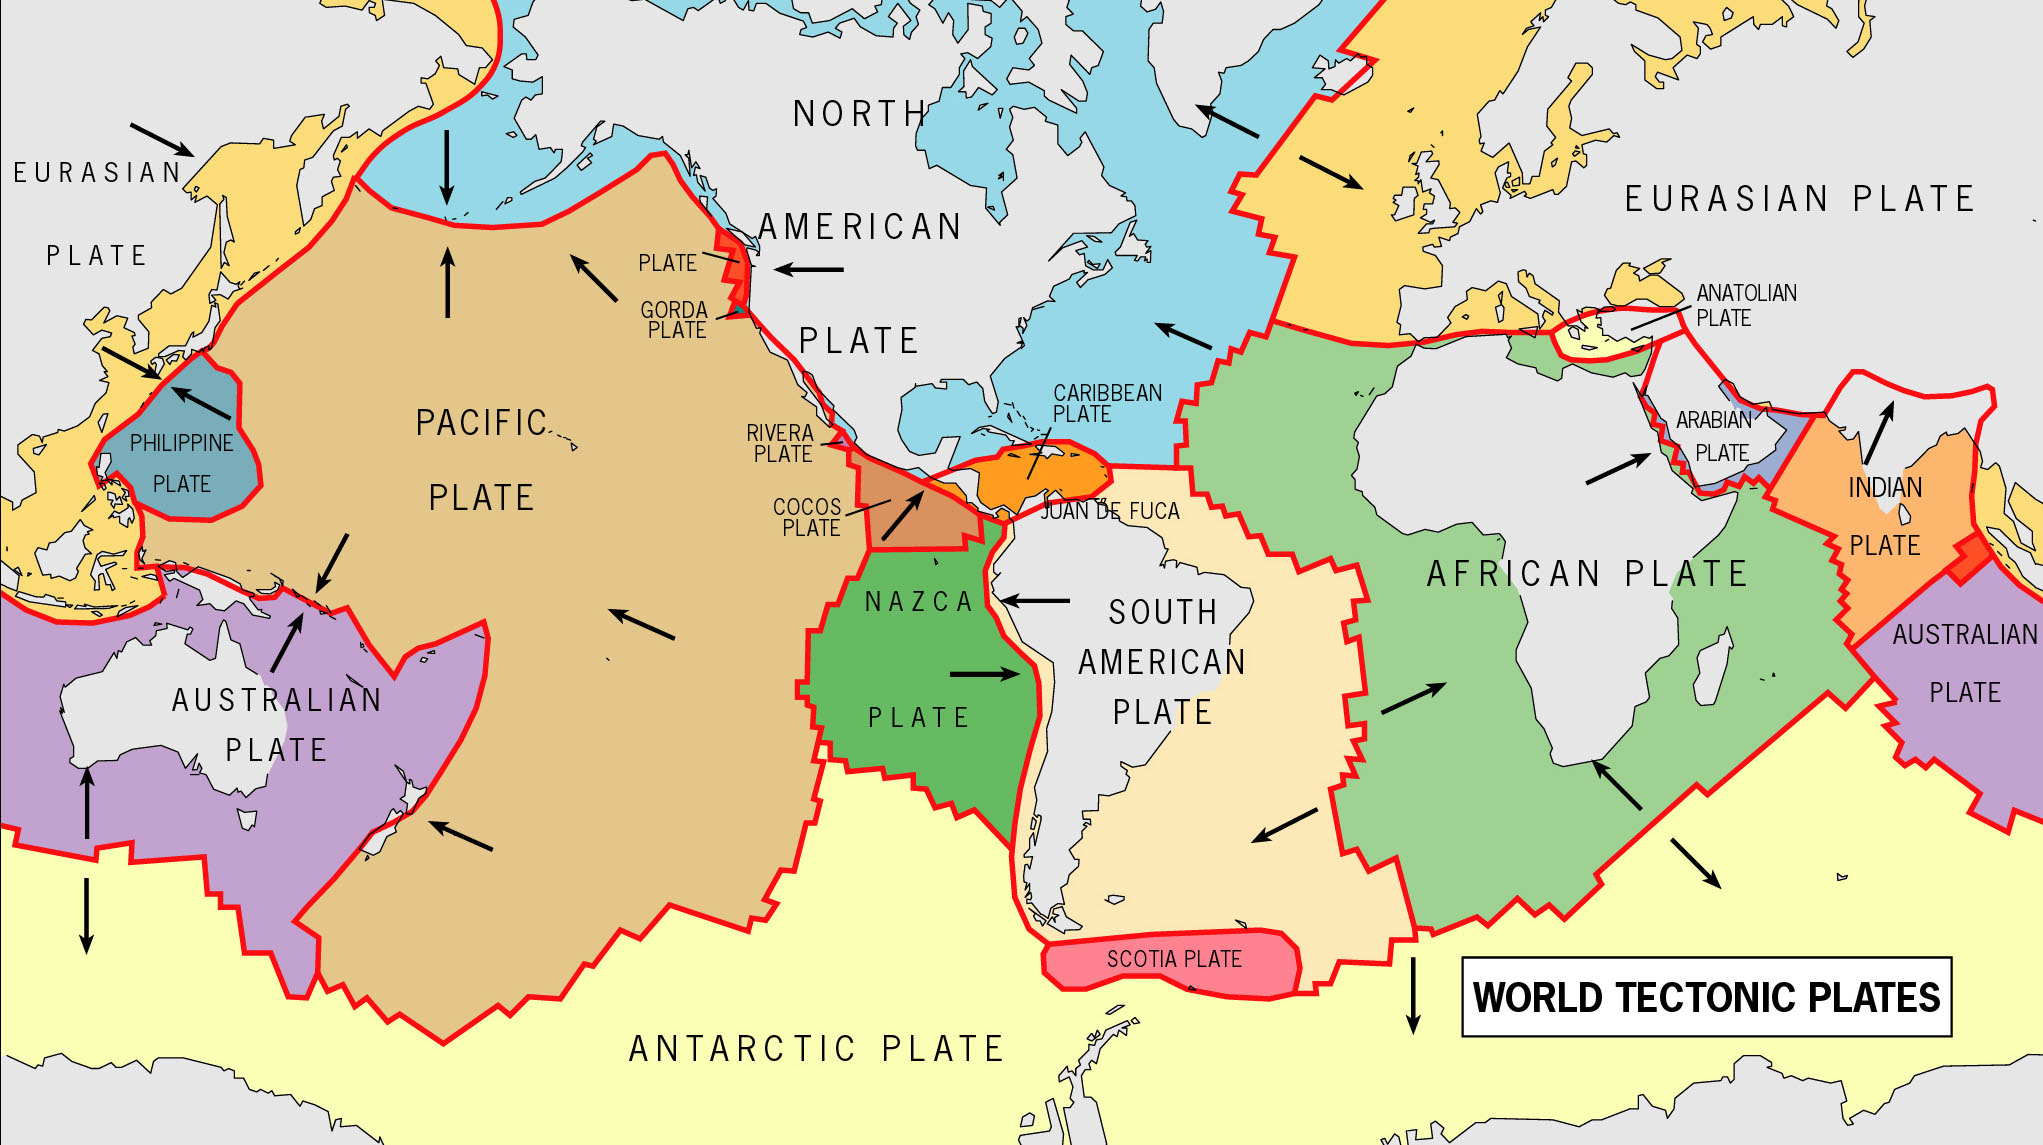
\includegraphics[keepaspectratio=true,width=0.8\paperwidth]{tectonic-plate}
\end{frame}
\begin{frame}
	\frametitle{Divisione dell'Italia nelle placche intercontinentali}
	\hspace{1em}
	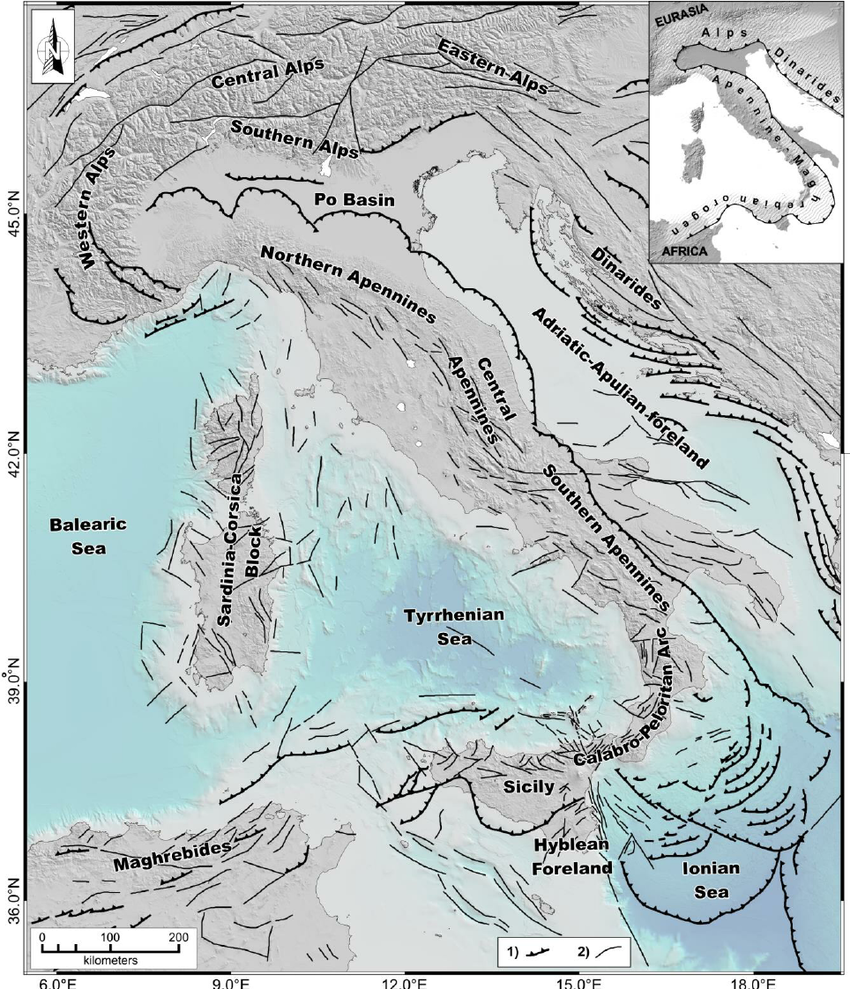
\includegraphics[keepaspectratio=true,height=0.8\paperheight]{italy-tectonic-map}
\end{frame}